\documentclass[11pt,oneside]{book}
\usepackage[utf8]{inputenc} 
\usepackage[T1]{fontenc} % fonts to encode unicode
%\usepackage{draftflag}
\usepackage{times}
\usepackage{fullpage}

\usepackage{makeidx}
\makeindex
\renewcommand{\indexname}{Author Index}

\usepackage{pdfpages}   % can also use [draft] option
\usepackage[colorlinks,
%%% EDIT TITLE: %%%%%%%%%%%%%%%%%%%%%%%%%%%%%%%%%%%%%%%%%%%%%%%%%%%%
            pdftitle={Proceedings of the IWCS Workshop on Models for Modality Annotation, MOMA 2015},
            pdfauthor={Association for Computational Linguistics},
            %pdfsubject={...},
            %pdfkeywords={...}
           ]{hyperref}   % hyperlinked table of contents, etc.
\hypersetup{plainpages=false}  % point to papers, not preface

% for Letter size %%%%%%%%%%%%%%%%%%%%%%%%%%%%%%%%%%%%%%%%%%%%%%%%%%%
%\special{papersize=8.5in,11in}
%\pdfpageheight\paperheight
%\pdfpagewidth\paperwidth
%\setlength\topmargin{-7mm} \setlength\oddsidemargin{-0cm}
%\setlength\textheight{22cm} \setlength\textwidth{15.8cm}
%\setlength\columnsep{0.25in}  \newlength\titlebox \setlength\titlebox{2.00in}
%\setlength\headheight{5pt}   \setlength\headsep{0pt}
%\setlength\footskip{1.9cm}
%\setlength\leftmargin{0.0in}
%\pagestyle{plain}
%%%%%%%%%%%%%%%%%%%%%%%%%%%%%%%%%%%%%%%%%%%%%%%%%%%

% for A4 size %%%%%%%%%%%%%%%%%%%%%%%%%%%%%%%%%%%%%%%%%%%%%%%%%%%
\setlength{\paperwidth}{21cm}   % A4
\setlength{\paperheight}{29.7cm}% A4
\special{papersize=21cm, 29.7cm}
\pdfpageheight\paperheight
\pdfpagewidth\paperwidth
\setlength\topmargin{-5mm} \setlength\oddsidemargin{-0cm}
\setlength\textheight{24.7cm} \setlength\textwidth{16cm}
\setlength\columnsep{0.6cm}  \newlength\titlebox \setlength\titlebox{2.00in}
\setlength\headheight{5pt}   \setlength\headsep{0pt}
\setlength\footskip{1.2cm}
\setlength\leftmargin{0.0in}
\pagestyle{plain}
%%%%%%%%%%%%%%%%%%%%%%%%%%%%%%%%%%%%%%%%%%%%%%%%%%%


\newcommand{\citeinfo}[2]{
  \AddToShipoutPicture{%
    \setlength{\unitlength}{1mm}
%%% EDIT NAME, DATES, LOCATION %%%%%%%%%%%%%%%%%%%%%%%%%%
    \put(105,11){\makebox(0,0){\footnotesize {\em Proceedings of the IWCS Workshop on Models for Modality Annotation, MOMA 2015}, 
	\ifthenelse{\equal{#1}{#2}}{page #1}{pages #1--#2},}}
     \put(105,8){\makebox(0,0){\footnotesize London, UK, April 14 2015. \copyright 2015 Association for Computational Linguistics}}
  }
}

% for Letter size %%%%%%%%%%%%%%%%%%%%%%%%%%%%%%%%%%%%%%%%%%%%%%%%%%%
%\newcommand{\draftframe}[1][0]{
% \AddToShipoutPicture{
%   \setlength{\unitlength}{1mm}
%    \put(20,28){\line(1,0){175}}
%    \put(20,259){\line(1,0){175}}
%    \multiput(20,239)(0,10){4}{\line(1,0){40}}
%    \multiput(20,239)(0,5){8}{\line(1,0){30}}
%    \multiput(20,239)(0,1){35}{\line(1,0){20}}
%
%    \put(70,239){\makebox(0,0){20mm}}
%    \put(70,249){\makebox(0,0){10mm}}
%    \put(70,269){\makebox(0,0){-10mm}}
%
%    \put(25,23){\line(0,1){251}}
%    \put(190,23){\line(0,1){251}}
%    \multiput(15,172)(10,0){3}{\line(0,1){53}}
%    \multiput(15,172)(5,0){5}{\line(0,1){46}}
%    \multiput(15,172)(1,0){20}{\line(0,1){40}}
%    \put(15,232){\makebox(0,0){-10}}
%    \put(35,232){\makebox(0,0){10}}
%    \put(15,227){\makebox(0,0){mm}}
%    \put(35,227){\makebox(0,0){mm}}
%
%    \put(108,264){\makebox(0,0){\bf \LARGE \tt Paper ID #1}}
%  }
%}

%%%%%%%%%%%%%%%%%%%%%%%%%%%%%%%%%%%%%%%%%%%%%%%%%%%


% for A4 size %%%%%%%%%%%%%%%%%%%%%%%%%%%%%%%%%%%%%%%%%%%%%%%%%%%

\newcommand{\draftframe}[1][0]{
  \AddToShipoutPicture{
    \setlength{\unitlength}{1mm}
    \put(20,25){\line(1,0){175}}
    \put(20,276){\line(1,0){175}}
    \multiput(20,256)(0,10){4}{\line(1,0){40}}
    \multiput(20,256)(0,5){8}{\line(1,0){30}}
    \multiput(20,256)(0,1){35}{\line(1,0){20}}
    \put(70,256){\makebox(0,0){20mm}}
    \put(70,266){\makebox(0,0){10mm}}
    \put(70,286){\makebox(0,0){-10mm}}

    \put(25,20){\line(0,1){271}}
    \put(186,20){\line(0,1){271}}

    \multiput(15,172)(10,0){3}{\line(0,1){53}}
    \multiput(15,172)(5,0){5}{\line(0,1){46}}
    \multiput(15,172)(1,0){20}{\line(0,1){40}}

    \put(15,232){\makebox(0,0){-10}}
    \put(35,232){\makebox(0,0){10}}
    \put(15,227){\makebox(0,0){mm}}
    \put(35,227){\makebox(0,0){mm}}

    \put(108,282){\makebox(0,0){\bf \LARGE \tt Paper ID #1}}
  }
}

%%%%%%%%%%%%%%%%%%%%%%%%%%%%%%%%%%%%%%%%%%%%%%%%%%%

\begin{document}
\pagenumbering{roman}

% -------- COVER --------

\thispagestyle{empty}
%\ifthenelse{\equal{\draftflag}{1}}{\draftframe}{}

\includepdf{titlepage.pdf}

% -------- FRONT MATTER --------

\includepdfset{pages=-,clip,noautoscale,pagecommand={\thispagestyle{plain}}}

%\ifthenelse{\equal{\draftflag}{1}}{\draftframe}{}
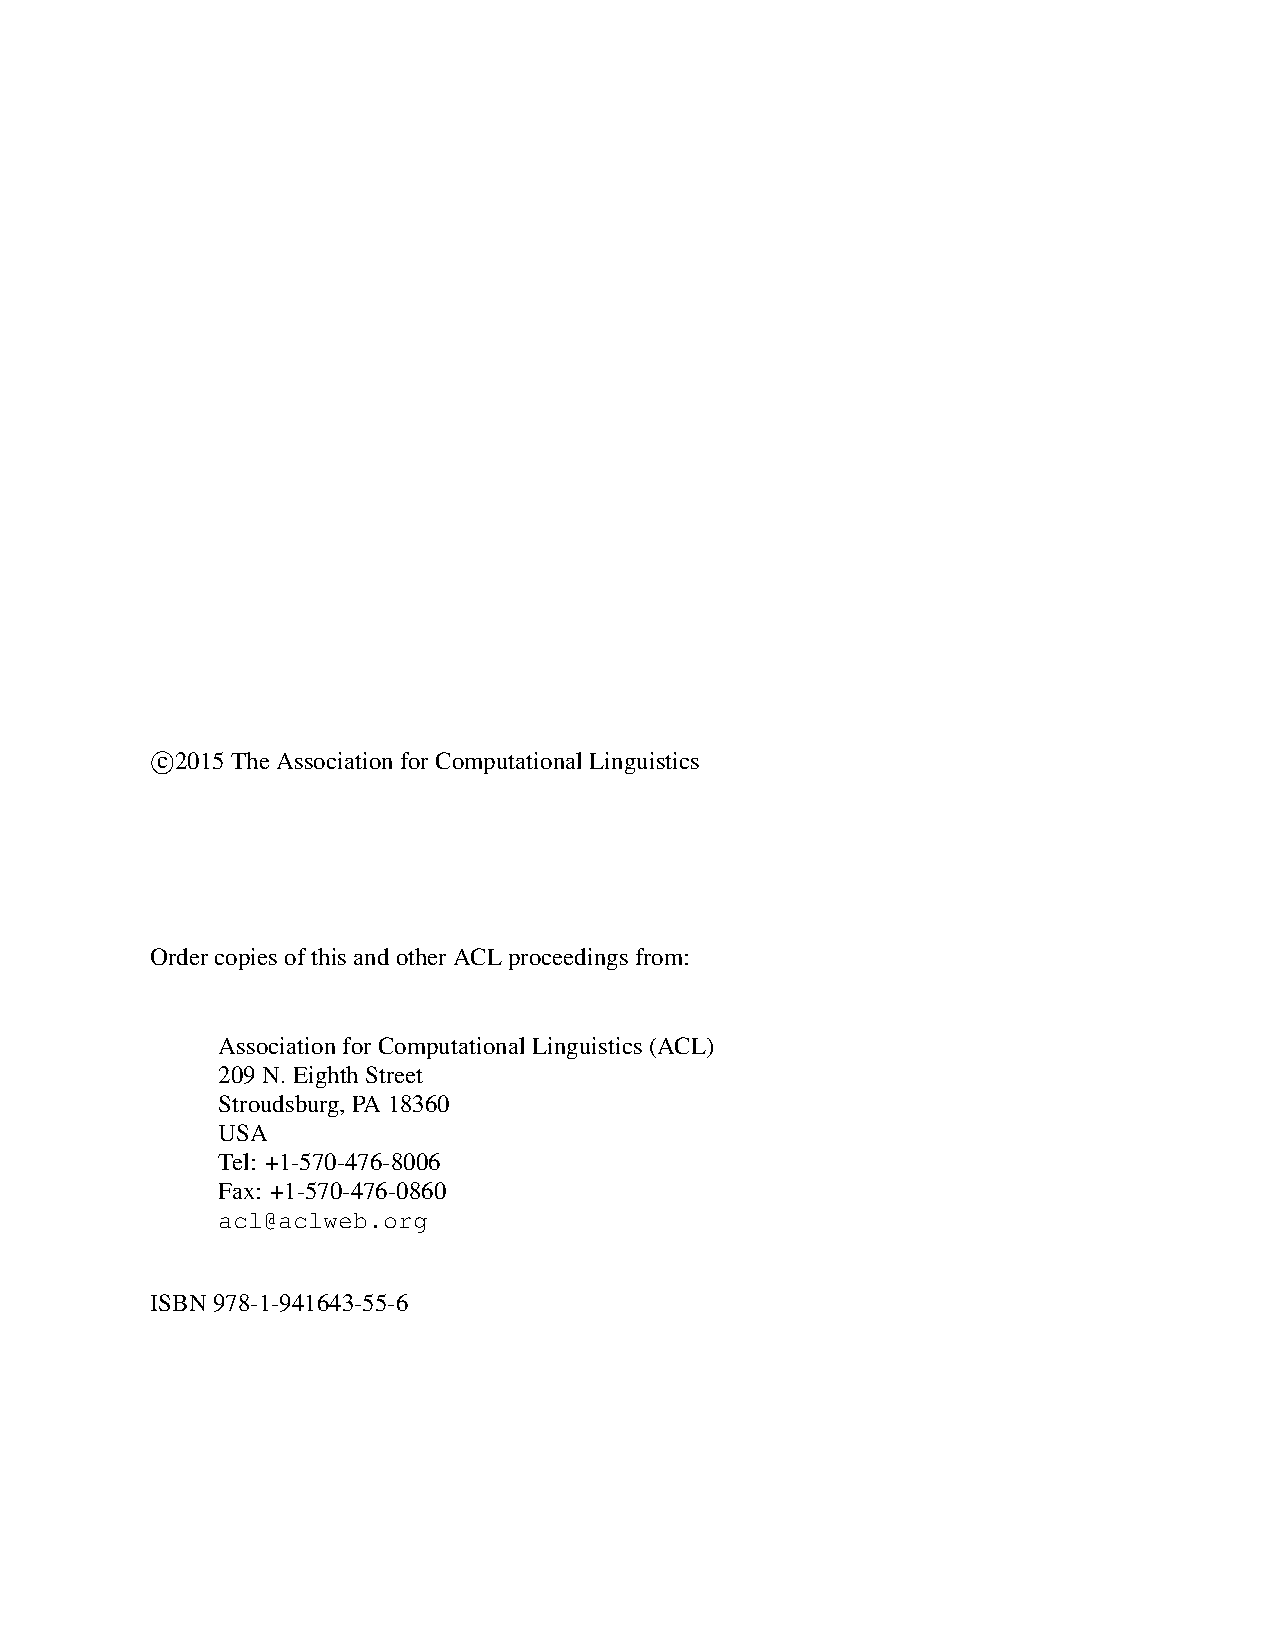
\includepdf{copyright.pdf}

%\ifthenelse{\equal{\draftflag}{1}}{\draftframe}{}
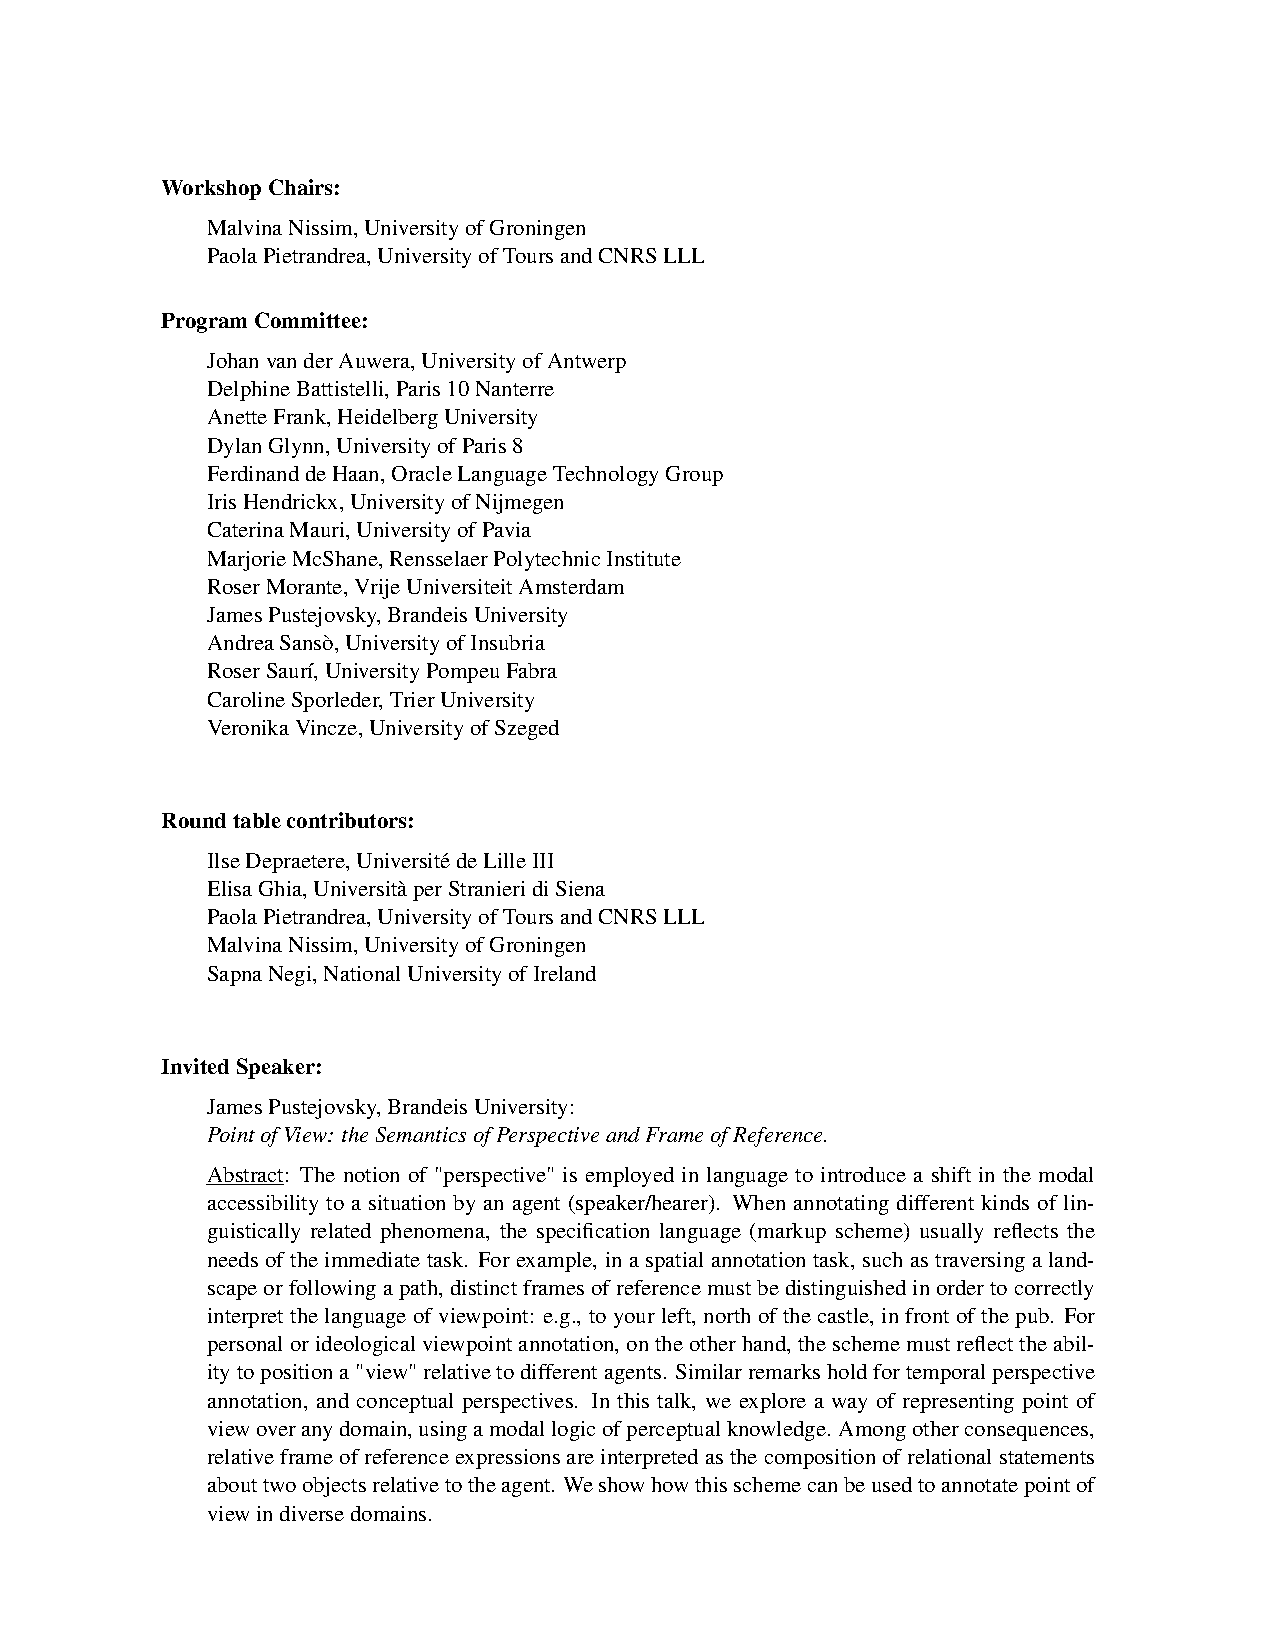
\includepdf{organizers.pdf}
\ifthenelse{\isodd{\value{page}}}{}{\newpage \thispagestyle{empty} \phantom{.}}

%\ifthenelse{\equal{\draftflag}{1}}{\draftframe}{}
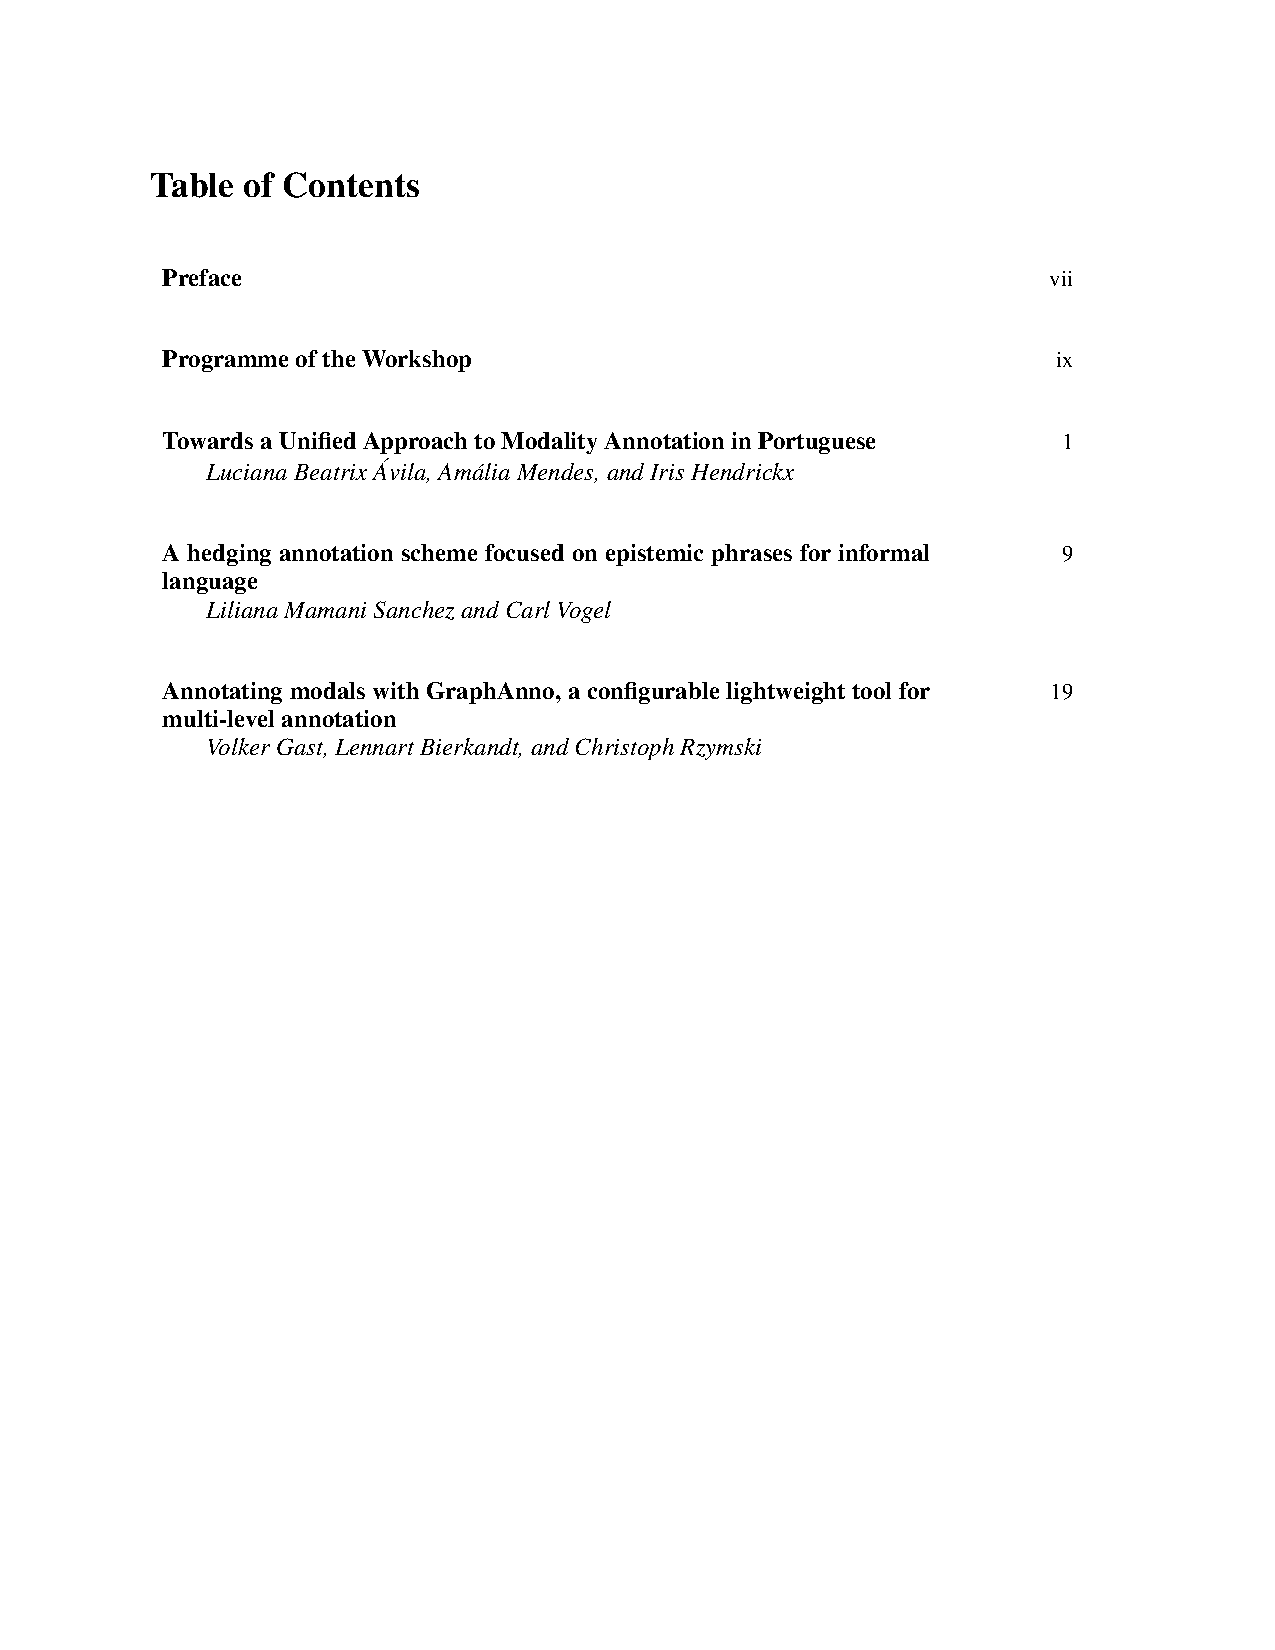
\includepdf{toc}
\ifthenelse{\isodd{\value{page}}}{}{\newpage \thispagestyle{empty} \phantom{.}}

%\ifthenelse{\equal{\draftflag}{1}}{\draftframe}{}
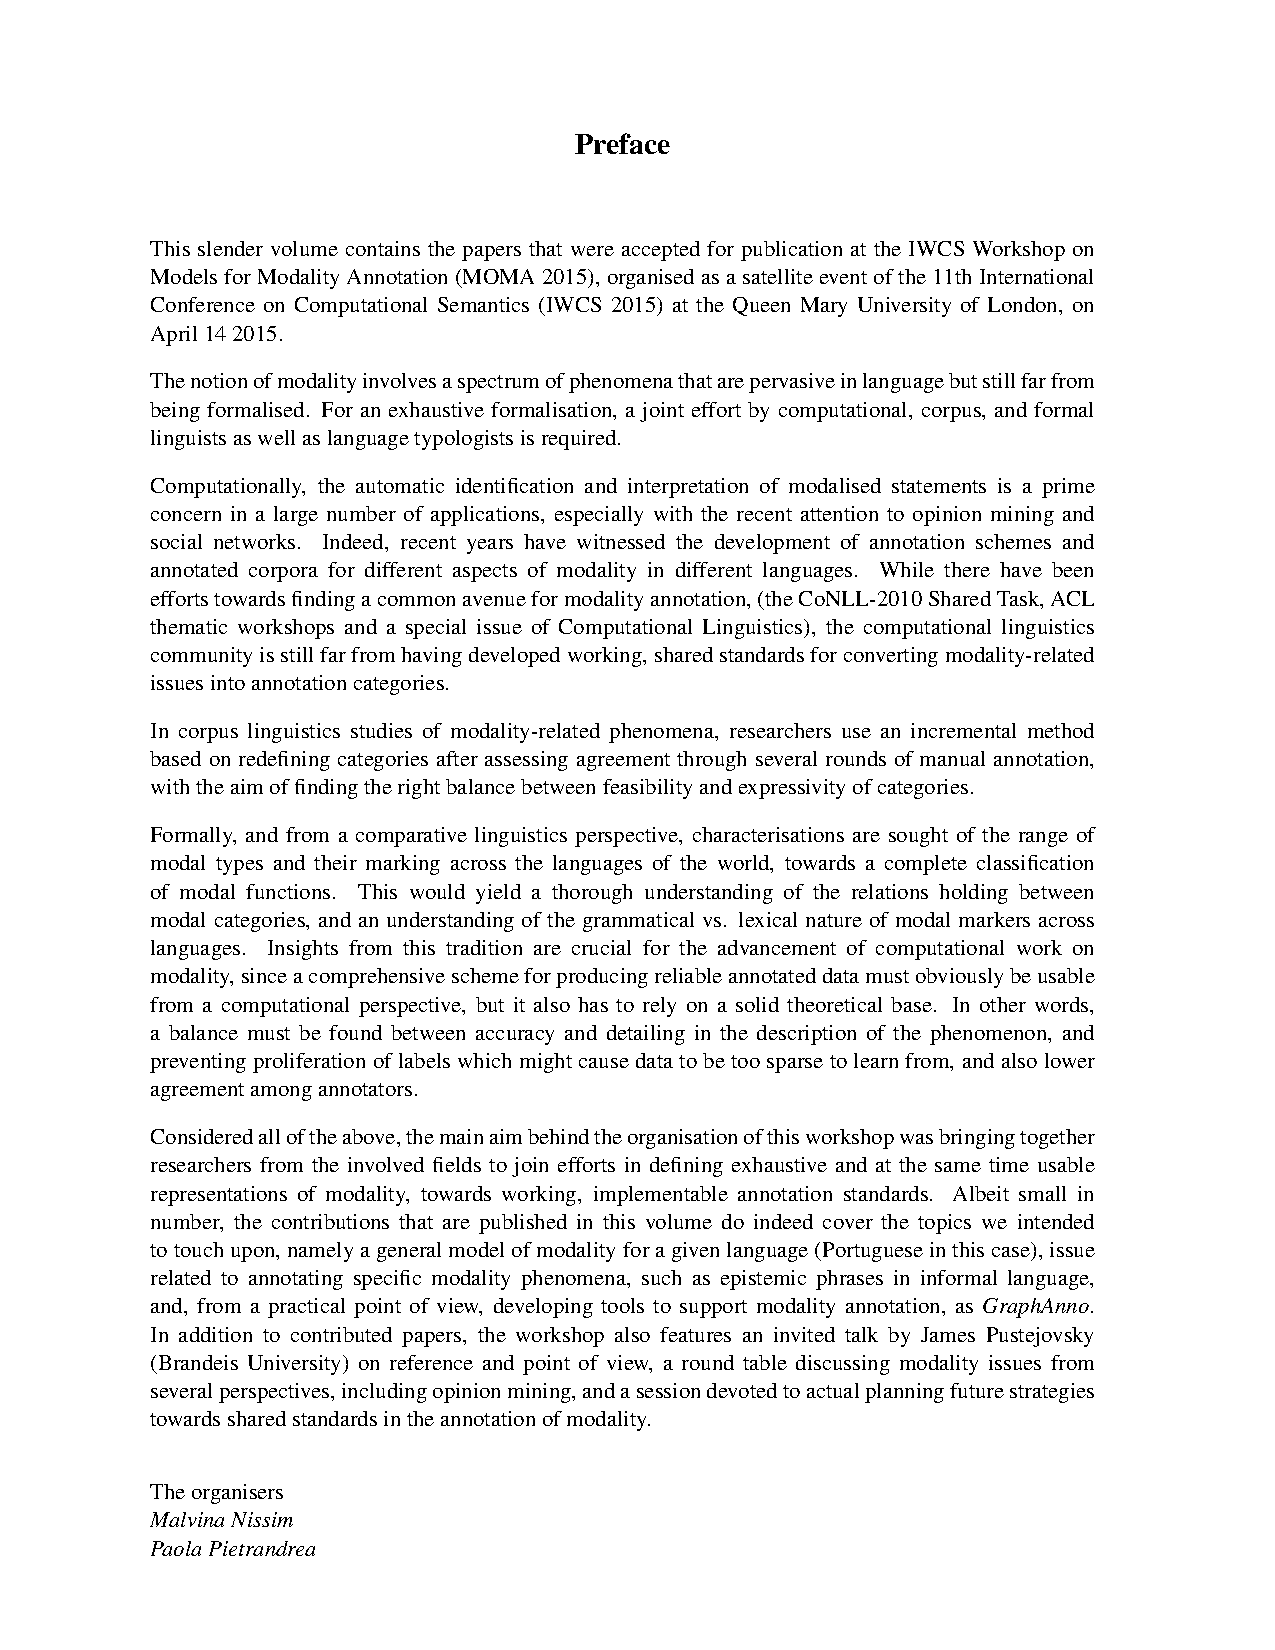
\includepdf{preface.pdf}
\ifthenelse{\isodd{\value{page}}}{}{\newpage \thispagestyle{empty} \phantom{.}}

%\tableofcontents

%\ifthenelse{\equal{\draftflag}{1}}{\draftframe}{}
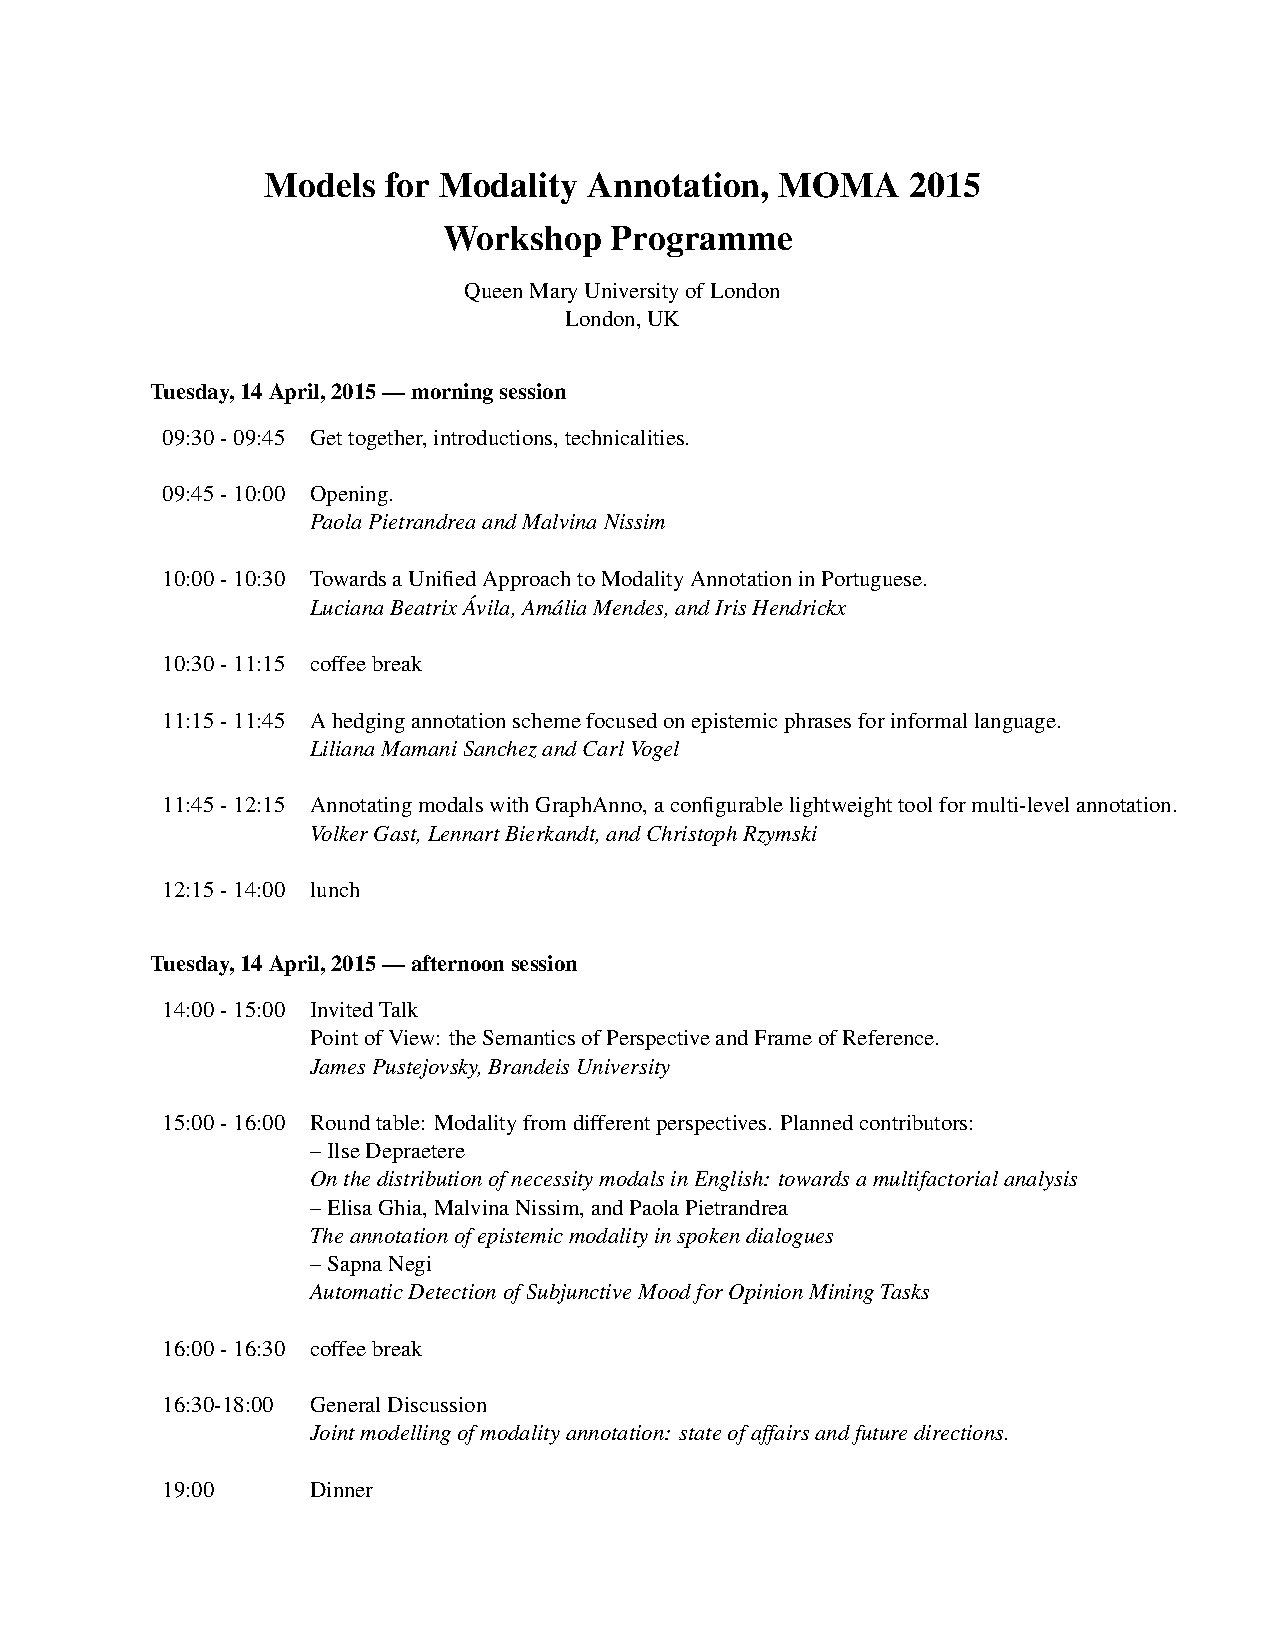
\includepdf{program.pdf}
\ifthenelse{\isodd{\value{page}}}{}{\newpage \thispagestyle{empty} \phantom{.}}

% -------- INCLUDED PAPERS --------

\newpage
\pagenumbering{arabic}
\setcounter{page}{1}
\ClearShipoutPicture

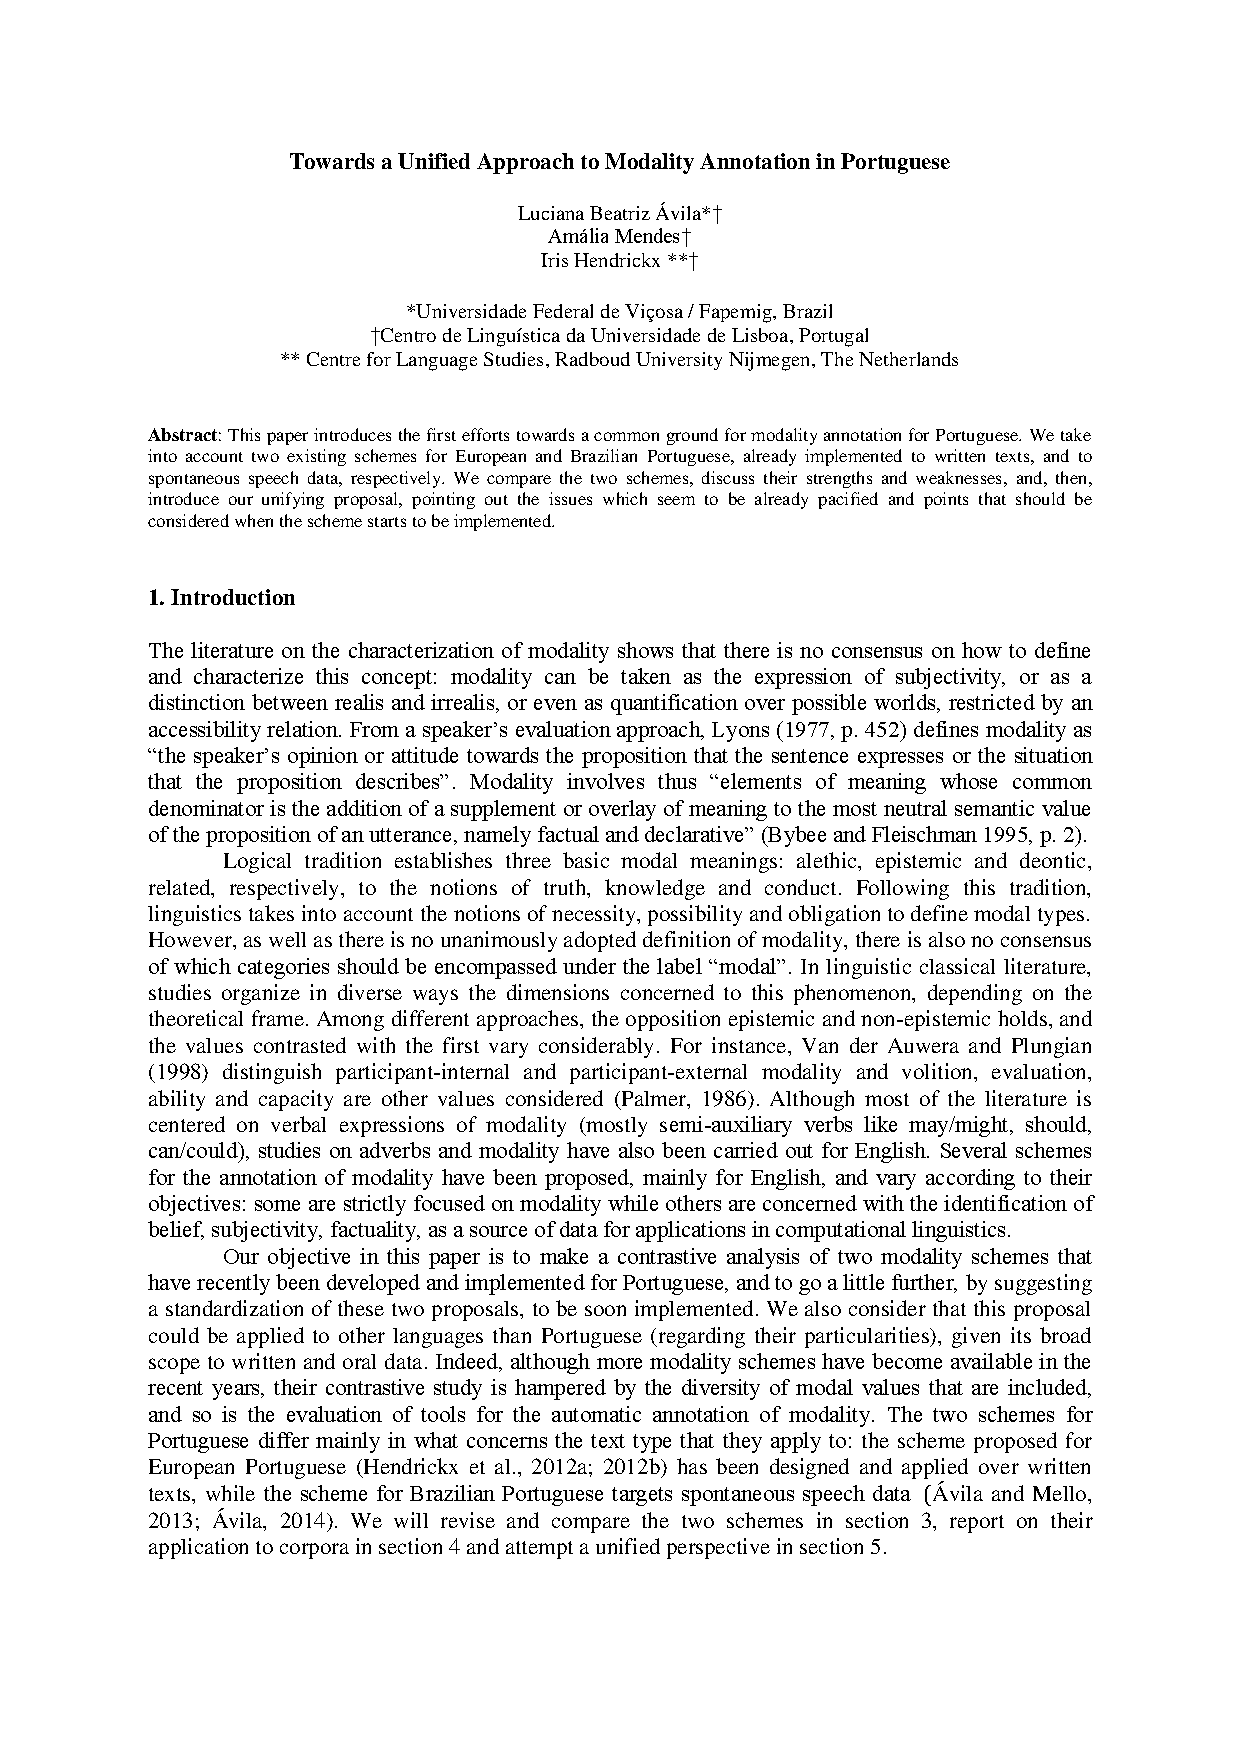
\includepdf{W15-0301}
\ifthenelse{\isodd{\value{page}}}{}{\newpage \thispagestyle{empty} \phantom{.}}

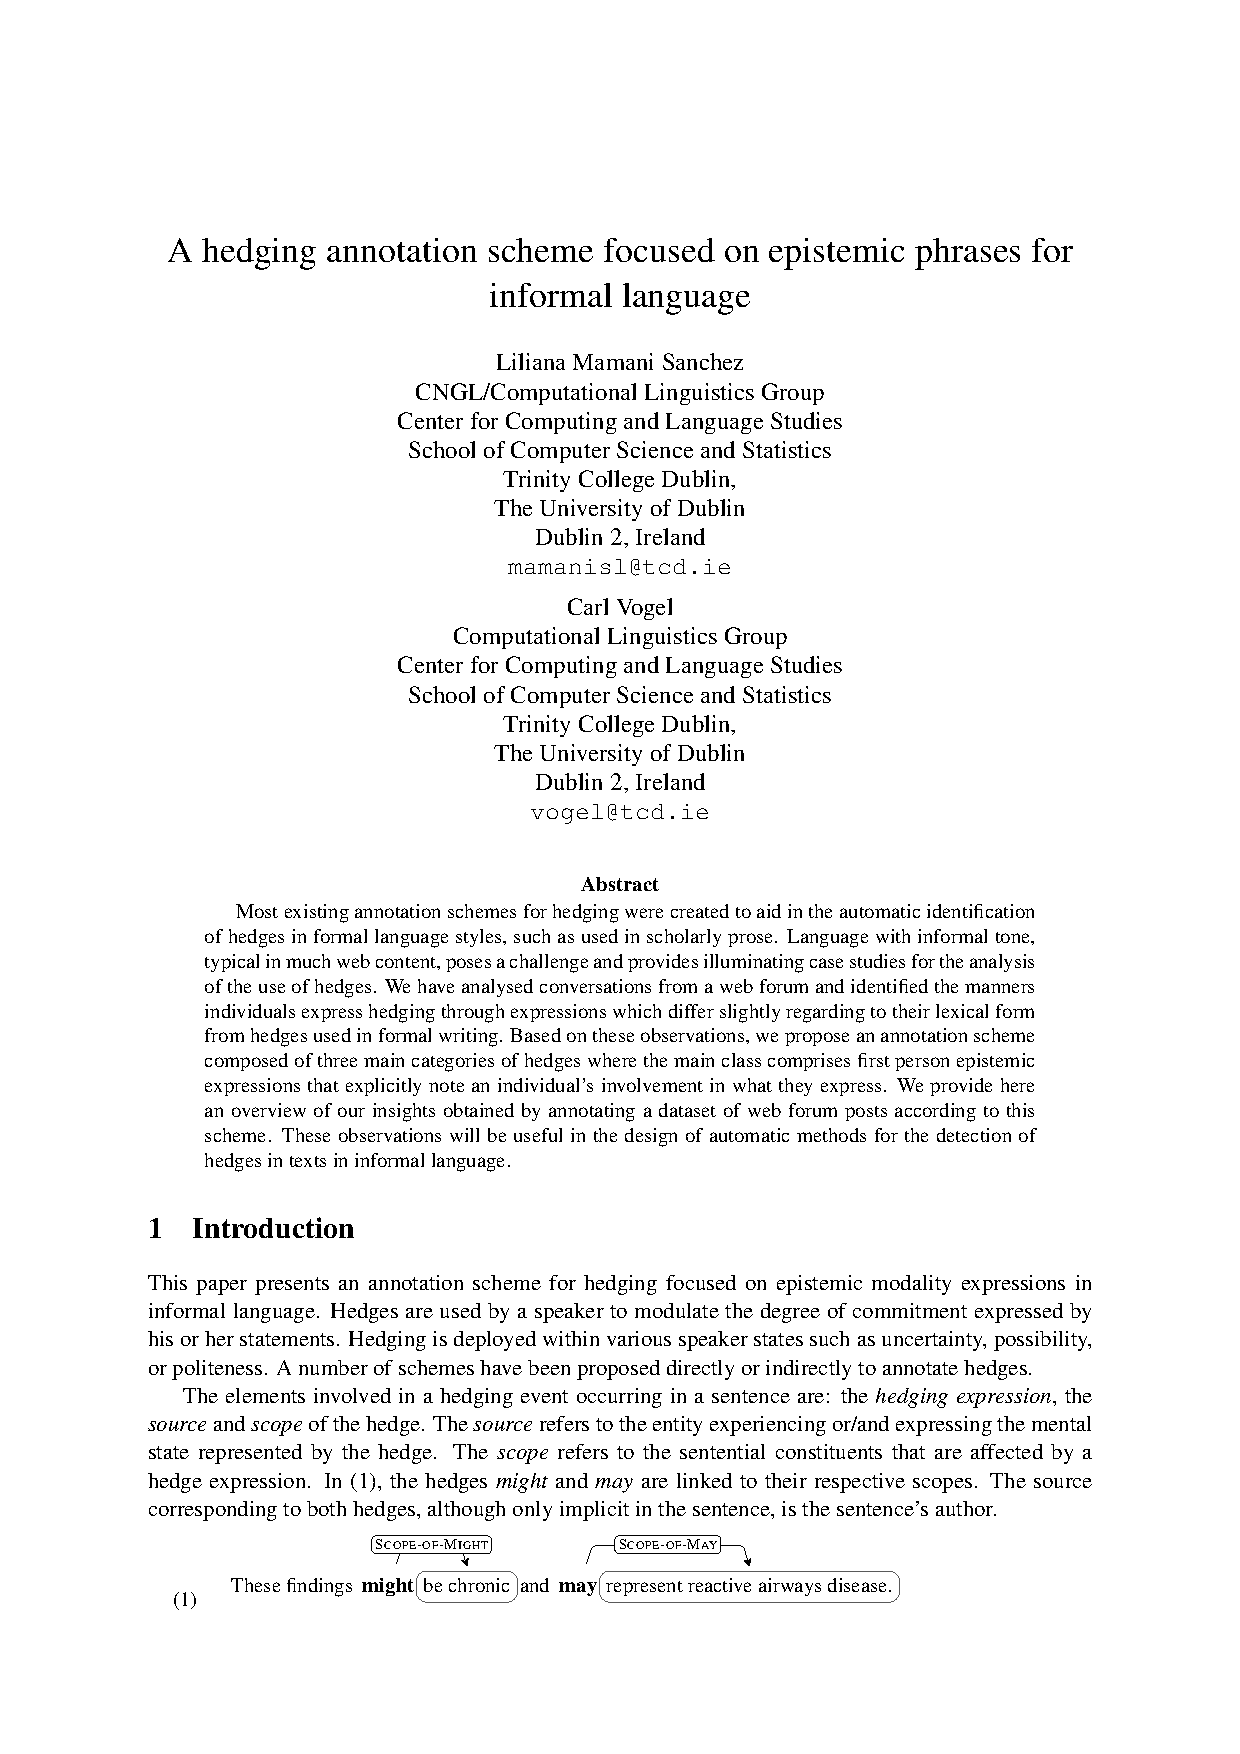
\includepdf{W15-0302}
\ifthenelse{\isodd{\value{page}}}{}{\newpage \thispagestyle{empty} \phantom{.}}

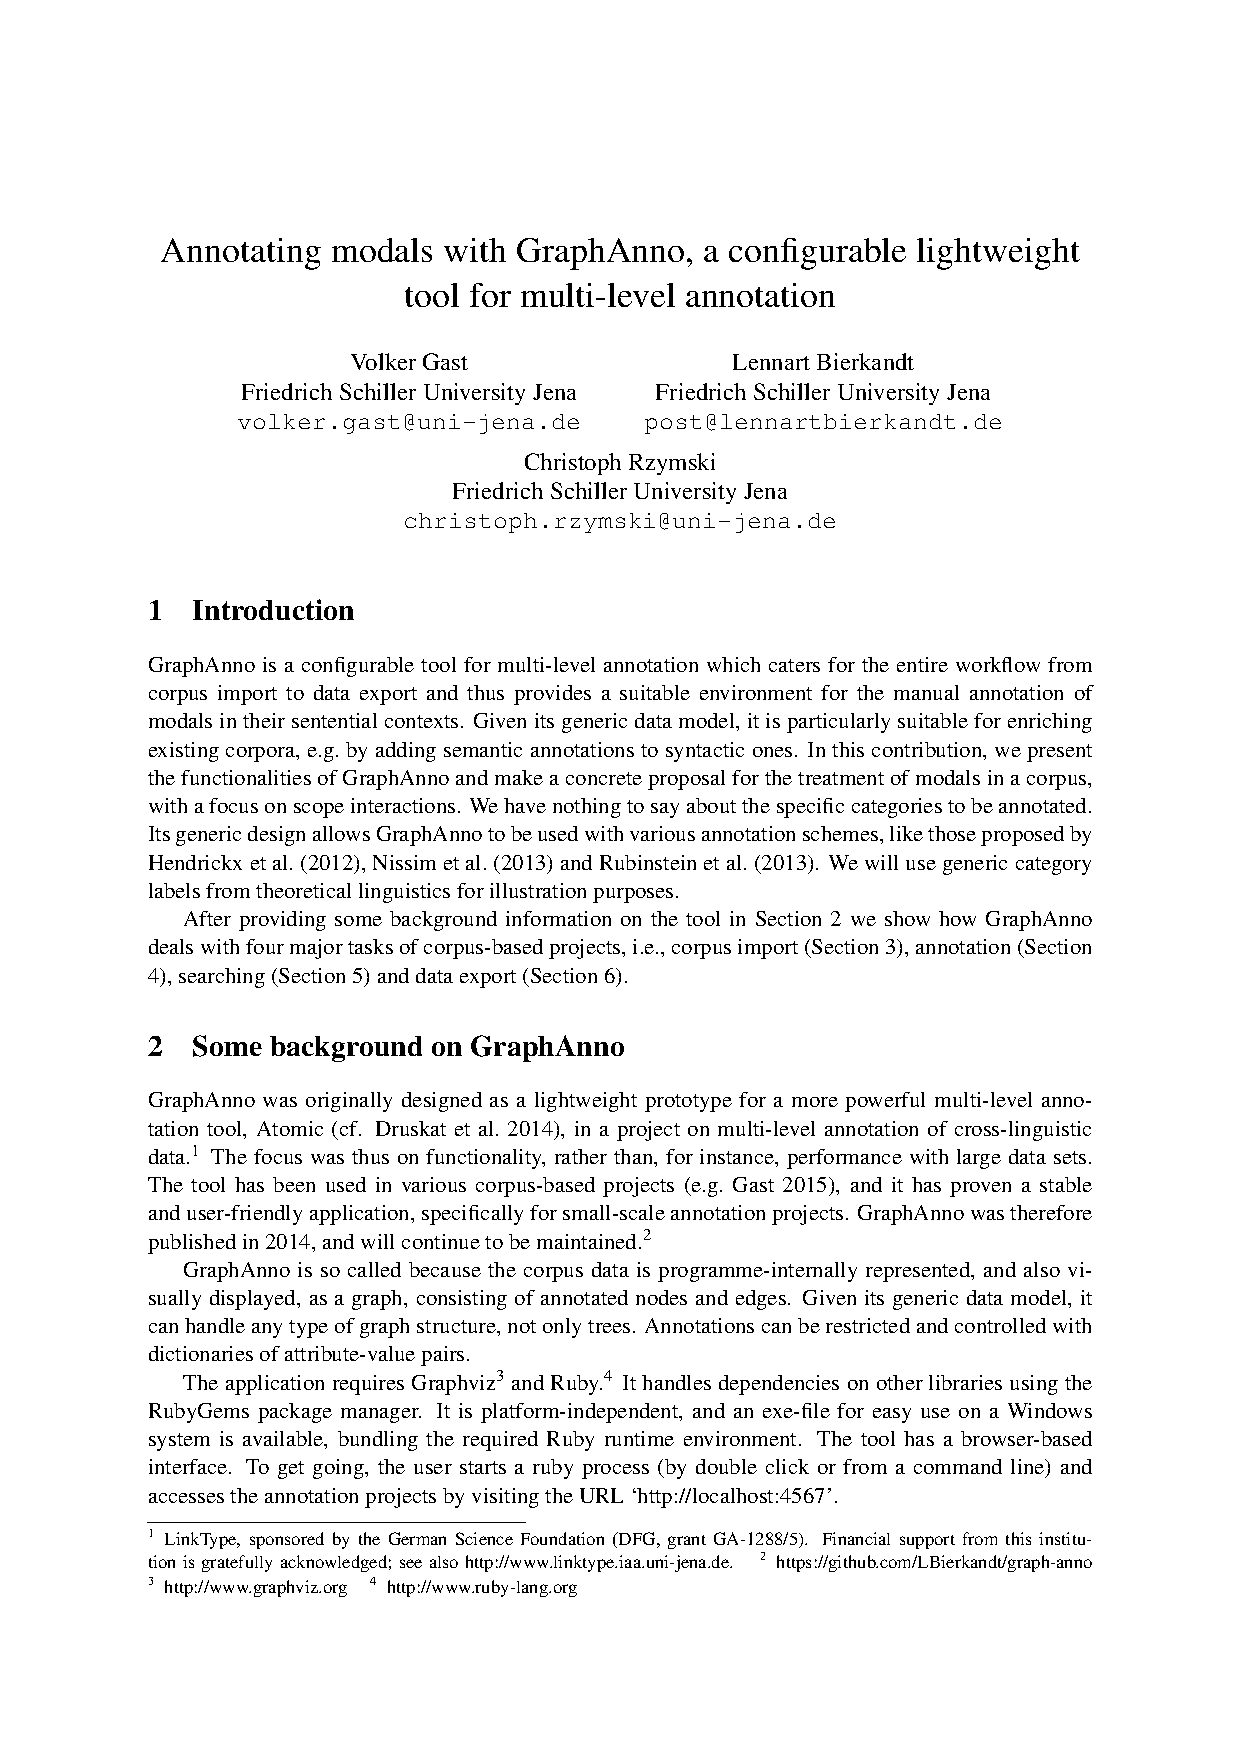
\includepdf{W15-0303}
\ifthenelse{\isodd{\value{page}}}{}{\newpage \thispagestyle{empty} \phantom{.}}

%\include{allpapers}   % automatically generated from DB file

% -------- END MATTER: AUTHOR INDEX --------

%\ifthenelse{\equal{\draftflag}{1}}{}{
  \ifthenelse{\isodd{\value{page}}}{}
    {\newpage \thispagestyle{empty} \phantom{.}}
  \pagestyle{empty}
  \printindex
%}

\end{document}
